% Created by tikzDevice version 0.7.0 on 2015-04-28 10:39:40
% !TEX encoding = UTF-8 Unicode
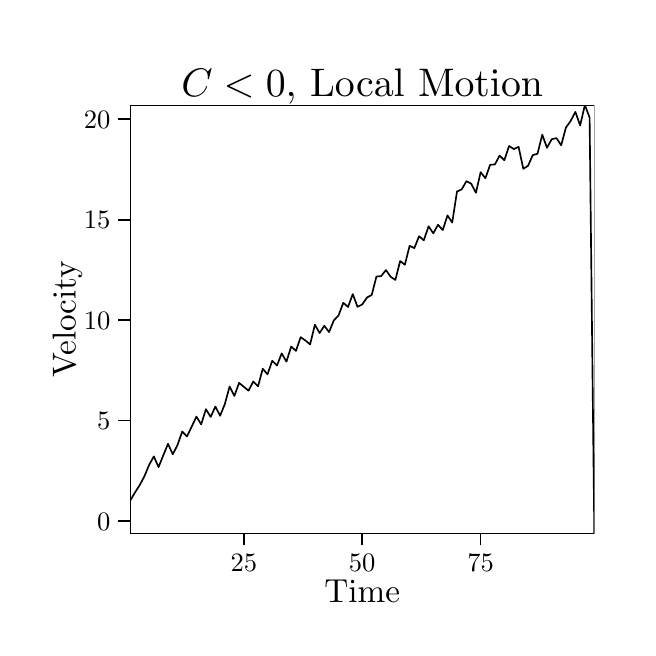
\begin{tikzpicture}[x=1pt,y=1pt]
\definecolor[named]{fillColor}{rgb}{1.00,1.00,1.00}
\path[use as bounding box,fill=fillColor,fill opacity=0.00] (0,0) rectangle (216.81,216.81);
\begin{scope}
\path[clip] (  0.00,  0.00) rectangle (216.81,216.81);
\definecolor[named]{drawColor}{rgb}{1.00,1.00,1.00}
\definecolor[named]{fillColor}{rgb}{1.00,1.00,1.00}

\path[draw=drawColor,line width= 0.6pt,line join=round,line cap=round,fill=fillColor] (  0.00,  0.00) rectangle (216.81,216.81);
\end{scope}
\begin{scope}
\path[clip] ( 37.02, 34.03) rectangle (204.76,188.82);
\definecolor[named]{fillColor}{rgb}{1.00,1.00,1.00}

\path[fill=fillColor] ( 37.02, 34.03) rectangle (204.76,188.82);
\definecolor[named]{drawColor}{rgb}{0.00,0.00,0.00}

\path[draw=drawColor,line width= 0.6pt,line join=round] ( 37.02, 45.88) --
	( 38.73, 48.76) --
	( 40.44, 51.45) --
	( 42.16, 54.66) --
	( 43.87, 58.79) --
	( 45.58, 61.89) --
	( 47.29, 58.01) --
	( 49.00, 62.26) --
	( 50.71, 66.44) --
	( 52.43, 62.65) --
	( 54.14, 66.01) --
	( 55.85, 70.87) --
	( 57.56, 69.09) --
	( 59.27, 72.66) --
	( 60.98, 76.26) --
	( 62.70, 73.48) --
	( 64.41, 78.94) --
	( 66.12, 76.16) --
	( 67.83, 79.91) --
	( 69.54, 76.57) --
	( 71.25, 80.81) --
	( 72.97, 87.16) --
	( 74.68, 83.73) --
	( 76.39, 88.45) --
	( 78.10, 87.05) --
	( 79.81, 85.64) --
	( 81.52, 88.96) --
	( 83.24, 87.19) --
	( 84.95, 93.57) --
	( 86.66, 91.54) --
	( 88.37, 96.45) --
	( 90.08, 94.73) --
	( 91.79, 99.11) --
	( 93.51, 96.13) --
	( 95.22,101.58) --
	( 96.93,100.01) --
	( 98.64,104.97) --
	(100.35,103.78) --
	(102.06,102.36) --
	(103.78,109.48) --
	(105.49,106.47) --
	(107.20,109.08) --
	(108.91,106.82) --
	(110.62,111.02) --
	(112.33,112.83) --
	(114.05,117.39) --
	(115.76,115.88) --
	(117.47,120.54) --
	(119.18,115.94) --
	(120.89,116.80) --
	(122.60,119.29) --
	(124.32,120.23) --
	(126.03,126.88) --
	(127.74,127.05) --
	(129.45,129.22) --
	(131.16,126.80) --
	(132.87,125.64) --
	(134.59,132.48) --
	(136.30,131.14) --
	(138.01,137.96) --
	(139.72,137.16) --
	(141.43,141.44) --
	(143.14,139.97) --
	(144.86,145.03) --
	(146.57,142.50) --
	(148.28,145.59) --
	(149.99,143.67) --
	(151.70,148.98) --
	(153.41,146.39) --
	(155.13,157.59) --
	(156.84,158.38) --
	(158.55,161.35) --
	(160.26,160.44) --
	(161.97,157.14) --
	(163.68,164.60) --
	(165.40,162.39) --
	(167.11,167.28) --
	(168.82,167.37) --
	(170.53,170.60) --
	(172.24,168.91) --
	(173.95,174.05) --
	(175.67,172.94) --
	(177.38,173.76) --
	(179.09,165.81) --
	(180.80,166.89) --
	(182.51,170.76) --
	(184.22,171.25) --
	(185.94,178.13) --
	(187.65,173.42) --
	(189.36,176.49) --
	(191.07,176.91) --
	(192.78,174.30) --
	(194.49,180.72) --
	(196.21,183.12) --
	(197.92,186.37) --
	(199.63,181.48) --
	(201.34,188.82) --
	(203.05,184.36) --
	(204.76, 34.03);

\path[draw=drawColor,line width= 0.6pt,line join=round,line cap=round] ( 37.02, 34.03) rectangle (204.76,188.82);
\end{scope}
\begin{scope}
\path[clip] (  0.00,  0.00) rectangle (216.81,216.81);
\definecolor[named]{drawColor}{rgb}{0.00,0.00,0.00}

\node[text=drawColor,anchor=base east,inner sep=0pt, outer sep=0pt, scale=  0.96] at ( 29.91, 35.19) {0};

\node[text=drawColor,anchor=base east,inner sep=0pt, outer sep=0pt, scale=  0.96] at ( 29.91, 71.49) {5};

\node[text=drawColor,anchor=base east,inner sep=0pt, outer sep=0pt, scale=  0.96] at ( 29.91,107.79) {10};

\node[text=drawColor,anchor=base east,inner sep=0pt, outer sep=0pt, scale=  0.96] at ( 29.91,144.10) {15};

\node[text=drawColor,anchor=base east,inner sep=0pt, outer sep=0pt, scale=  0.96] at ( 29.91,180.40) {20};
\end{scope}
\begin{scope}
\path[clip] (  0.00,  0.00) rectangle (216.81,216.81);
\definecolor[named]{drawColor}{rgb}{0.00,0.00,0.00}

\path[draw=drawColor,line width= 0.6pt,line join=round] ( 32.75, 38.50) --
	( 37.02, 38.50);

\path[draw=drawColor,line width= 0.6pt,line join=round] ( 32.75, 74.80) --
	( 37.02, 74.80);

\path[draw=drawColor,line width= 0.6pt,line join=round] ( 32.75,111.10) --
	( 37.02,111.10);

\path[draw=drawColor,line width= 0.6pt,line join=round] ( 32.75,147.40) --
	( 37.02,147.40);

\path[draw=drawColor,line width= 0.6pt,line join=round] ( 32.75,183.70) --
	( 37.02,183.70);
\end{scope}
\begin{scope}
\path[clip] (  0.00,  0.00) rectangle (216.81,216.81);
\definecolor[named]{drawColor}{rgb}{0.00,0.00,0.00}

\path[draw=drawColor,line width= 0.6pt,line join=round] ( 78.10, 29.77) --
	( 78.10, 34.03);

\path[draw=drawColor,line width= 0.6pt,line join=round] (120.89, 29.77) --
	(120.89, 34.03);

\path[draw=drawColor,line width= 0.6pt,line join=round] (163.68, 29.77) --
	(163.68, 34.03);
\end{scope}
\begin{scope}
\path[clip] (  0.00,  0.00) rectangle (216.81,216.81);
\definecolor[named]{drawColor}{rgb}{0.00,0.00,0.00}

\node[text=drawColor,anchor=base,inner sep=0pt, outer sep=0pt, scale=  0.96] at ( 78.10, 20.31) {25};

\node[text=drawColor,anchor=base,inner sep=0pt, outer sep=0pt, scale=  0.96] at (120.89, 20.31) {50};

\node[text=drawColor,anchor=base,inner sep=0pt, outer sep=0pt, scale=  0.96] at (163.68, 20.31) {75};
\end{scope}
\begin{scope}
\path[clip] (  0.00,  0.00) rectangle (216.81,216.81);
\definecolor[named]{drawColor}{rgb}{0.00,0.00,0.00}

\node[text=drawColor,anchor=base,inner sep=0pt, outer sep=0pt, scale=  1.20] at (120.89,  9.03) {Time};
\end{scope}
\begin{scope}
\path[clip] (  0.00,  0.00) rectangle (216.81,216.81);
\definecolor[named]{drawColor}{rgb}{0.00,0.00,0.00}

\node[text=drawColor,rotate= 90.00,anchor=base,inner sep=0pt, outer sep=0pt, scale=  1.20] at ( 17.30,111.43) {Velocity};
\end{scope}
\begin{scope}
\path[clip] (  0.00,  0.00) rectangle (216.81,216.81);
\definecolor[named]{drawColor}{rgb}{0.00,0.00,0.00}

\node[text=drawColor,anchor=base,inner sep=0pt, outer sep=0pt, scale=  1.44] at (120.89,191.84) {$C < 0$, Local Motion};
\end{scope}
\end{tikzpicture}
